%%%
\subsection{Data-Level Techniques for Imbalanced Data}

Consider this two-dimensional training dataset, which we will use to illustrate data-level techniques for handling imbalanced datasets.  In real problems, of course, the dataset could have a hundred dimensions and a million samples.  The six blue circles represent samples (elements) of the majority negative class (``no ambulance''), and the three red squares represent the minority positive class (``ambulance'').  


\begin{center}
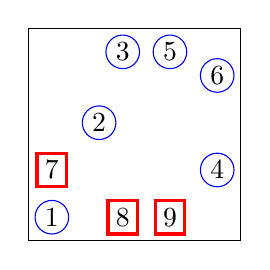
\begin{tikzpicture}[x = 3mm, y=3mm]
	\draw (-1,-1) rectangle (8,8);
	\tikzstyle{Square} = [
		draw = red, 
		very thick,
		rectangle,
		inner sep = 1mm,
		minimum size = 2 mm
	]
	\tikzstyle{SquareFill} = [
		draw = red, 
		fill = red,
		very thick,
		rectangle,
	]
	\tikzstyle{Circle} = [
		draw = blue, 
		circle,		
		inner sep = 0.5mm,
	]
	\tikzstyle{CircleFill} = [
		draw = blue,
		fill = blue, 
		circle,
	]
	\node [Circle] (1) at (0,0) {1};
	\node [Circle] (2) at (2,4) {2};
	\node [Circle] (3) at (3,7) {3};
	\node [Circle] (4) at (7,2) {4};
	\node [Circle] (5) at (5,7) {5};
	\node [Circle] (6) at (7,6) {6};
	\node [Square] (7) at (0,2) {7};
	\node [Square] (8) at (3,0) {8};
	\node [Square] (9) at (5,0) {9};

\end{tikzpicture}
\end{center}

Many algorithms, and variations thereon, have been proposed to balance the two classes before applying a machine learning algorithm to build a model to classify new samples as positive or negative.  WARNING:  Vast oversimplification ahead.  Our goal here is to give the general idea of each method.  



\subsubsection{Random Undersampling}

Random undersampling balances the two classes by randomly deleting elements of the majority class until the two are balanced.  The major drawback of this method is that you throw away information about the majority class.  If the majority class is many more times the size of the minority, you lose almost all of the data.  


\begin{center}
\begin{tikzpicture}[x = 3mm, y=3mm]
	\draw (-1,-1) rectangle (8,8);
	\tikzstyle{Square} = [
		draw = red, 
		very thick,
		rectangle,
		inner sep = 1 mm,
		minimum size = 3 mm
	]
	\tikzstyle{SquareFill} = [
		draw = red, 
		fill = red,
		very thick,
		rectangle,
	]
	\tikzstyle{Circle} = [
		draw = blue, 
		circle,
		inner sep = 0.5 mm
	]
	\tikzstyle{CircleFill} = [
		draw = blue,
		fill = blue, 
		circle,
	]
	\node [Circle] (1) at (0,0) {1};
	\node [Circle] (2) at (2,4) {2};
	\node [Circle] (3) at (3,7) {3};
	\node [Circle] (4) at (7,2) {4};
	\node [Circle] (5) at (5,7) {5};
	\node [Circle] (6) at (7,6) {6};
	\node [Square] (7) at (0,2) {7};
	\node [Square] (8) at (3,0) {8};
	\node [Square] (9) at (5,0) {9};

	\node [Circle, cross out] (1) at (0,0) {1};
	\node [Circle, cross out] (4) at (7,2) {4};
	\node [Circle, cross out] (6) at (7,6) {6};
\end{tikzpicture}
\end{center}

\subsubsection{Random Oversampling}

Random oversampling creates duplicates of minority class samples until the sets are balanced.  This method has a similar effect to using class weights, introduced below.  

\begin{center}
\begin{tikzpicture}[x = 3mm, y=3mm]
	\draw (-1,-1) rectangle (8,8);
	\tikzstyle{Square} = [
		draw = red, 
		very thick,
		rectangle,
		inner sep = 1mm,
		minimum size = 4 mm
	]
	\tikzstyle{SquareFill} = [
		draw = red, 
		fill = red,`	
		very thick,
		rectangle,
	]
	\tikzstyle{Circle} = [
		draw = blue, 
		circle,
		inner sep = 0.5 mm
	]
	\tikzstyle{CircleFill} = [
		draw = blue,
		fill = blue, 
		circle,
	]
	\node [Circle] (1) at (0,0) {1};
	\node [Circle] (2) at (2,4) {2};
	\node [Circle] (3) at (3,7) {3};
	\node [Circle] (4) at (7,2) {4};
	\node [Circle] (5) at (5,7) {5};
	\node [Circle] (6) at (7,6) {6};
	\node [Square] (7) at (0,2) {7};
	\node [Square] (8) at (3,0) {8};
	\node [Square] (9) at (5,0) {9};

%	\node [Square] (7) at ($(0,2) + (-0.2,-0.2)$) {};
	\node [Square] (8) at ($(3,0) + (-0.2,-0.2)$) {};
%	\node [Square] (9) at ($(5,0) + (-0.2,-0.2)$) {};

%	\node [Square] (7) at ($(0,2) + (0.2,0.2)$) {};
	\node [Square] (8) at ($(3,0) + (0.2,0.2)$) {};
	\node [Square] (9) at ($(5,0) + (0.2,0.2)$) {};


\end{tikzpicture}
\end{center}

%%%
\subsubsection{Synthetic Minority Sampling TEchnique (SMOTE)}

SMOTE \citep{00017602530000120020101} is one of the most popular oversampling methods for balancing a dataset with continuous numerical data.  It creates new synthetic minority samples ``between'' original minority samples, not necessarily at the midpoint by choosing a number in $(0,1)$, multiplying the difference (in each dimension) from point $A$ to $B$ by that constant, and adding it to $A$.

In the diagram, the solid red squares represent new synthetic samples between pairs of original minority-class samples.  SMOTE does not consider the positions of the majority-class samples, only considering the difference in number of nodes to bring the two classes closer to parity.  

\begin{center}
\begin{tikzpicture}[x = 7mm, y=7mm]
%	\draw (-1,-1) rectangle (8,8);
	\tikzstyle{Square} = [
		draw = red, 
		very thick,
		rectangle,
		minimum size = 5 mm
	]
	\tikzstyle{Synth} = [
		draw = red, 
		fill = red,
		very thick,
		rectangle,
		minimum size = 3mm
	]
	\tikzstyle{Circle} = [
		draw = blue, 
		circle,
	]
	\tikzstyle{CircleFill} = [
		draw = blue,
		fill = blue, 
		circle,
	]
	\node [Square] (7) at (0,2) {7};
	\node [Square] (8) at (3,0) {8};
	\node [Square] (9) at (5,0) {9};

	\draw (7) -- (8);
	\draw (7) -- (9);
	\draw (8) -- (9);
	
	\node [Synth] () at ($0.3*(7) + 0.7*(8)$) {};
	\node [Synth] () at ($0.7*(7) + 0.3*(9)$) {};
	\node [Synth] () at ($0.5*(8) + 0.5*(9)$) {};


\end{tikzpicture}
\end{center}

One challenge with SMOTE is that it is only useful for datasets with continuous numerical data, and our data is almost all categorical.  What is between ``car'' and ``school bus,'' or between ``parking lot'' and ``highway''?  SMOTE has a variant, SMOTE-NC (Nominal and Continuous) that can handle datasets with some nominal (categorical) features, but most of the features need to be continuous; thus, we will not be able to use SMOTE or similar techniques for our work.  


%%%
\subsubsection{Tomek's Links}

\cite{ivan1976two} proposed a method of undersampling that assumes that the majority and minority classes should (at least locally) be clustered.  If an sample $A$ of the majority class and a sample $B$ of the minority class are each other's nearest neighbors, then one of them is not clustered with its own class.  Since we are trying to undersample the majority class, assume that the element of the majority class is noise (or an error, or just not useful), and delete it.  

In the diagram below, samples \#1 and \#7 are Tomek links, because they are each other's nearest neighbors and of different classes.  Samples \#4 and \#9 are not Tomek links, because while 9 is 4's nearest neighbor, 9's nearest neighbor is 8, not 4.  

In the context of modeling crash severity from police reports, why would sample \#1 not need an ambulance when its characteristics are so close to those of \#7 and not near most of the other crashes without serious injury?  The reason could be errors in the records, or luck/providence/fate.  It could also be that the difference between property damage only and serious injury is influenced by thousands of variables we cannot measure or know, all of the physics of crash forces acting on the bones and structures of the human body.  The best we can say is that the outcome in \#1 cannot be predicted by the information that we have, so that sample will not help in constructing a model based on the available data; therefore, we can reasonably delete it from the training set.  

Tomek's Links can also be run iteratively.  Sample \#7 had \#1 as its nearest neighbor, but once \#1 is deleted, then \#2 and \#7 are each other's nearest neighbors of different classes, thus are Tomek links, and we can delete \#2.  



\begin{center}
\begin{tikzpicture}[x = 3mm, y=3mm]
	\draw (-1,-1) rectangle (8,8);
	\tikzstyle{Square} = [
		draw = red, 
		very thick,
		rectangle,
		inner sep = 1mm,
		minimum size = 3 mm
	]
	\tikzstyle{SquareFill} = [
		draw = red, 
		fill = red,
		very thick,
		rectangle,
	]
	\tikzstyle{Circle} = [
		draw = blue, 
		circle,
		inner sep = 0.5 mm
	]
	\tikzstyle{CircleFill} = [
		draw = blue,
		fill = blue, 
		circle,
	]
	\node [Circle] (1) at (0,0) {1};
	\node [Circle] (2) at (2,4) {2};
	\node [Circle] (3) at (3,7) {3};
	\node [Circle] (4) at (7,2) {4};
	\node [Circle] (5) at (5,7) {5};
	\node [Circle] (6) at (7,6) {6};
	\node [Square] (7) at (0,2) {7};
	\node [Square] (8) at (3,0) {8};
	\node [Square] (9) at (5,0) {9};

	\node [Circle, cross out] (1) at (0,0) {1};
\end{tikzpicture}
\end{center}



%%%
\subsubsection{Oversampling Image Data}

Extracting knowledge from a database of tabular numerical or categorical data is difficult, but a database of images is a challenge of a different magnitude.  An imbalanced labeled image dataset for crash prediction modeling might be a thousand images taken ten seconds before a crash and a million images taken ten seconds before ... nothing happened.  Deep neural networks (DNN) and (deep) convolutional neural networks (DCNN and CNN) are common methods for image data.  \cite{NIPS2014_5ca3e9b1} introduced Generative Adversarial Networks, which can be used to generate synthetic samples to balance the dataset.  Given the power of the tools for image recognition, many researchers make non-image data look (to the computer) like images to take advantage of the tools.  

